\documentclass[a4paper,10pt]{article}
\usepackage[utf8]{inputenc}
\usepackage[T1]{fontenc}
\usepackage{amsmath}
\usepackage{amsfonts}
\usepackage{amssymb}
\usepackage{booktabs}
\usepackage{etoolbox}
\usepackage{tikz}
\usepackage{xcolor}
\usepackage{geometry}
\usepackage{ragged2e}
\usepackage{environ}
\usepackage{framed}
\usepackage{graphicx}

% Neue Geometrie-Einstellungen für A4
\geometry{
	a4paper,
	margin=2.5cm,
	top=3cm,
	bottom=3cm,
	headheight=1.5cm,
	footskip=1.5cm
}

% Farben definieren
\definecolor{formulaColor}{RGB}{20,50,150}
\definecolor{legendColor}{RGB}{60,60,60}
\definecolor{formulabgcolor}{gray}{0.95}

% Neue Umgebung für Formeln
\newenvironment{displayformula}
{
	\begin{framed}
		\color{formulaColor}
	}
	{\end{framed}}

% Befehl für Formelerklärungen
\newcommand{\formulalegend}[1]{%
	\par\vspace{0.5ex}%
	{{\color{legendColor}\RaggedRight\small\textit{#1}}}%
	\par\vspace{1.5ex}%
}

\setcounter{tocdepth}{3}


\begin{document}
	\tableofcontents
	
	
	\section{Physikalische Größen und Einheiten}
	
	\subsection{Umrechnungen in SI-Einheiten}
	

		\begin{displayformula}
		\[
		\text{Kraft} F = kg \cdot \frac{m}{s^2} = N
		\]
		\[
		\text{Arbeit} W = kg \cdot \frac{m}{s^2} \cdot m = kg \cdot \frac{m^2}{s^2} = J
		\]
		\[
		\text{Leistung} P = \frac{kg \cdot m^2}{s^3} = W
		\]
		\[
		\text{Spannung} U = \frac{kg \cdot m^2}{s^2 \cdot As} = \frac{kg \cdot m^2}{A \cdot s^3} = V
		\]
		\[
		\text{Kapazität} C = \frac{A^2 \cdot s^4}{kg \cdot m^2} = \frac{C}{V} = \frac{As}{V} = F
		\]
		\[
		\text{Geschwindigkeit} v = \frac{m}{s}
		\]
		\[
		\text{Beschleunigung} a = \frac{m}{s^2}
		\]
		\end{displayformula}

	
	
	\subsection{Messunsicherheit Typ A}
	
	\begin{displayformula}
		Arithmetischer Mittelwert
		\[
		\bar{x} = \frac{1}{N} \sum_{i=1}^{N} x_i
		\]
	\end{displayformula}
	\formulalegend{
		\( \bar{x} \): Mittelwert der Messwerte [Einheit wie \( x_i \)], \( x_i \): Einzelne Messwerte, \( N \): Anzahl der Messungen
	}
	
	\begin{displayformula}
		Standartabweichung des Messverfahrens
		\[
		\Delta x = \sqrt{\frac{1}{N - 1} \sum_{i = 1}^{N} (x_i - \bar{x})}
		\]
	\end{displayformula}
		\formulalegend{
		\( \Delta x \): Standardabweichung [Einheit wie \( x_i \)], \( x_i \): Einzelne Messwerte, \( \bar{x} \): Mittelwert, \( N \): Anzahl der Messwerte
	}
	
	\begin{displayformula}
		Standartabweichung eines Messwertes
		\[
		\Delta x = \frac{1}{N - 1} \sum_{i = 1}^{N} (x_i - \bar{x})^2
		\]	
	\end{displayformula}
	\formulalegend{
		\( \Delta x \): Standardabweichung [Einheit wie \( x_i \)], \( x_i \): Einzelne Messwerte, \( \bar{x} \): Mittelwert, \( N \): Anzahl der Messwerte
	}
	
	\begin{displayformula}
		Standartabweichung des Mittelwertes
		\[
		\Delta \bar{x} = \frac{\Delta x}{\sqrt{N}} 
		\]	
	\end{displayformula}
	\formulalegend{
		\( \Delta \bar{x} \): Standardabweichung des Mittelwertes, \( \Delta x \): Standardabweichung [Einheit wie \( x_i \)], \( N \): Anzahl der Messwerte
	}
	
	\begin{displayformula}
		Darstellung der Messgröße x
		\[
		x_p = \bar{x} \pm t_p \cdot \Delta x
		\]
		\[
		x_p = \bar{x} \pm U_a (x)
		\]
	\end{displayformula}
	\formulalegend{
		\( x_p \): Messgröße, \( \bar{x} \): Mittelwert, \( t_p \): Vertrauensfaktor, \( \Delta x \): Standardabweichung, \( U_a(x) \): erweiterte Unsicherheit
	}
	
	\subsection{Messunsicherheit Typ B}
	\begin{displayformula}
		Unsicherheiten, welche nicht durch Wiederholungsmessungen ermittelt werden. \\ Die Messunsicherheit ist angegeben
	\end{displayformula}
	
	\subsubsection{Ermittlung des kombinierten Unsicherheit}
	
	\begin{displayformula}
		Wenn Typ A und Typ B vorliegen
		\[
		U_\text{mess} = \sqrt{U^2_A(x) + U^2_{B_1}(x) + U^2_{B_2}(x) + \dots}
		\]
	\end{displayformula}
	\formulalegend{
		\( U_\text{mess} \): Gesamte kombinierte Unsicherheit, \( U_A(x) \): Unsicherheit Typ A, \( U_{B_i}(x) \): Unsicherheit Typ B
	}
	
	\begin{displayformula}
		Bei Abhängigkeit mehrerer Größen (z.B. Volumen = abc)
		\[
		u_{ges} = \sqrt{(\frac{\partial_z}{\partial_a} \cdot \Delta a)^2 + (\frac{\partial_z}{\partial_b} \cdot \Delta b)^2 + (\frac{\partial_z}{\partial_c} \cdot \Delta c)^2 }
		\]
	\end{displayformula}
	
	
\section{Verschiebung, Geschwindigkeit und \\Geschwindigkeitsbetrag}

\begin{displayformula}
	Verschiebung
	\[
	\Delta x = x_E - x_A
	\]
\end{displayformula}
\formulalegend{
	\( \Delta x \): Verschiebung [m], \( x_E \): Endposition [m], \( x_A \): Anfangsposition [m]
}

\begin{displayformula}
	Mittlere Geschwindigkeit
	\[
	\bar{v}_x = \frac{\Delta x}{\Delta t}
	\]
\end{displayformula}
\formulalegend{
	\( \bar{v_x} \): Mittlere Geschwindigkeit [m/s], \( \Delta x \): Weg [m], \( \Delta t \): Zeitintervall [s]
}

\begin{displayformula}
	Momentangeschwindigkeit
	\[
	v_x = \dfrac{x}{t} = \dot{x} (t)
	\]
\end{displayformula}
\formulalegend{
	\( v_x \): Momentangeschwindigkeit [m/s], \( x \): Position [m], \( t \): Zeit [s], \( \dot{x}(t) \): Ableitung von \( x(t) \) nach der Zeit
}



\section{Gleichförmig beschleunigte Bewegung}

\begin{displayformula}
	Der mittlere Geschwindigkeitsbetrag (speed) \( \bar{v}_x \) ist definiert als zurückgelegte Strecke \( s \) geteilt durch die benötigte Zeit \( \Delta t \):
	\[
	\bar{v}_x = \frac{s}{\Delta t}
	\]
\end{displayformula}
\formulalegend{
	\( \bar{v}_x \): Mittlere Geschwindigkeit [m/s], \( s \): Strecke [m], \( \Delta t \): Zeitintervall [s]
}

\begin{displayformula}
	Die mittlere Beschleunigung \( \bar{a}_x \) ist definiert als Änderung der Geschwindigkeit \( v_x \) pro Zeiteinheit \( \Delta t \):
	\[
	\bar{a}_x = \frac{v_{xE} - v_{xA}}{\Delta t} = \frac{\Delta v_x}{\Delta t}
	\]
\end{displayformula}
\formulalegend{
	\( \bar{a}_x \): Mittlere Beschleunigung [m/s²], \( v_{xE} \): Endgeschwindigkeit [m/s], \( v_{xA} \): Anfangsgeschwindigkeit [m/s], \( \Delta t \): Zeit [s]
}



\section{Gleichmäßig beschleunigte Bewegung}

\begin{displayformula}
	\[
	x(t) = x_0 + v_{x0}t + \frac{1}{2} a_x t^2 
	\]
	\[
	v_x(t) = v_{x0} + a_x t
	\]
	\[
	a_x(t) = a_x
	\]
\end{displayformula}
\formulalegend{
	\( x(t) \): Position zur Zeit \( t \) [m], \( x_0 \): Anfangsposition [m], \( v_{x0} \): Anfangsgeschwindigkeit [m/s], \( a_x \): konstante Beschleunigung [m/s²], \( t \): Zeit [s]
}

\section{Bewegung in zwei und drei Dimensionen}

\begin{displayformula}
	\[
	r(t) = x(t)\vec{e_x} + y(t)\vec{e_y}
	\]
	\[
	= \begin{pmatrix}
		x(t) \\
		y(t)
	\end{pmatrix}
	\]
\end{displayformula}
\formulalegend{
	\( r(t) \): Ortsvektor [m], \( x(t), y(t) \): Komponenten der Position [m], \( \vec{e_x}, \vec{e_y} \): Einheitsvektoren
}

\begin{displayformula}
	\[
	\Delta \vec{r}(t) = \vec{r_E}(t) - \vec{r_A}(t)
	\]
	\[
	= \begin{pmatrix}
		x_E(t) - x_A(t) \\
		y_E(t) - y_A(t)
	\end{pmatrix}
	\]
\end{displayformula}
\formulalegend{
	\( \Delta \vec{r}(t) \): Verschiebungsvektor [m], \( \vec{r_E}(t) \): Endposition, \( \vec{r_A}(t) \): Anfangsposition
}

\begin{displayformula}
	Mittlere Geschwindigkeit
	\[
	\vec{v} = \frac{\Delta \vec{r}}{\Delta t}
	\]
\end{displayformula}
\formulalegend{
	\( \vec{v} \): Mittlere Geschwindigkeit [m/s], \( \Delta \vec{r} \): Verschiebung [m], \( \Delta t \): Zeitintervall [s]
}

\begin{displayformula}
	\[
	\vec{r}(t) = x(t)\vec{e_x} + y(t)\vec{e_y} + z(t)\vec{e_z}
	\]
	\[
	=
	\begin{pmatrix}
		x(t)\\
		y(t) \\
		z(t)
	\end{pmatrix}
	\]
	z.B.
	\[
	\vec{r}(t) = \begin{pmatrix}
		x_0 + v_{x0}t + \frac{1}{2}a_x t^2 \\
		y_0 + v_{y0}t + \frac{1}{2}a_y t^2 \\
		z_0 + v_{z0}t + \frac{1}{2}a_z t^2 
	\end{pmatrix}
	\]
\end{displayformula}
\formulalegend{
	\( \vec{r}(t) \): Ortsvektor [m], \( x_0, y_0, z_0 \): Anfangskoordinaten [m], \( v_{x0}, v_{y0}, v_{z0} \): Anfangsgeschwindigkeiten [m/s], \( a_x, a_y, a_z \): Beschleunigungen [m/s²], \( t \): Zeit [s]
}


\subsection{Der schräge Wurf}

\begin{displayformula}
	\[
	\vec{r}(t) =
	\begin{pmatrix}
		v_0 \cdot \cos\alpha \cdot t\\
		y_0 + v_0\sin\alpha \cdot t - \frac{1}{2} \cdot g \cdot t^2
	\end{pmatrix}
	=
	\begin{pmatrix}
		v_{x0} t\\
		y_0 + v_{y0} t - \frac{1}{2} g t^2
	\end{pmatrix}
	\]
\end{displayformula}
\formulalegend{
	\( \vec{r}(t) \): Ortsvektor [m], \( v_0 \): Anfangsgeschwindigkeit [m/s], \( \alpha \): Abwurfwinkel, \( g \): Erdbeschleunigung [m/s²], \( t \): Zeit [s], \( y_0 \): Anfangshöhe [m]
}

\begin{displayformula}
	\[
	y(t) = y_0 + v_0\sin\alpha \cdot t - \frac{1}{2} gt^2
	\]
\end{displayformula}
\formulalegend{
	\( y(t) \): Höhe zur Zeit \( t \) [m], \( y_0 \): Anfangshöhe [m], \( v_0 \): Anfangsgeschwindigkeit [m/s], \( \alpha \): Winkel, \( g \): Erdbeschleunigung [m/s²], \( t \): Zeit [s]
}

\begin{displayformula}
	\[
	y(x) = y_0 + v_0\sin\alpha \cdot \frac{x}{v_0 \cos\alpha} - \frac{1}{2} g \left(\frac{x}{v_0\cos\alpha}\right)^2
	\]
\end{displayformula}
\formulalegend{
	\( y(x) \): Höhe in Abhängigkeit vom horizontalen Ort \( x \) [m], \( y_0 \): Anfangshöhe [m], \( v_0 \): Anfangsgeschwindigkeit [m/s], \( \alpha \): Winkel, \( g \): Erdbeschleunigung [m/s²], \( x \): horizontale Entfernung [m]
}



\section{Die Newtonschen Axiome}

\begin{displayformula}
	\[
	F = m \cdot a
	\]
\end{displayformula}
\formulalegend{
	\( F \): Kraft [N], \( m \): Masse [kg], \( a \): Beschleunigung [m/s²]
}

\subsection{Das erste Newtonsche Axiom: Das Trägheitsgesetz}

\begin{displayformula}
	Ein Körper bleibt in Ruhe oder bewegt sich geradlinig mit konstanter Geschwindigkeit weiter, wenn keine resultierende Kraft auf ihn wirkt
	\[
	\vec{a} = 0 \quad \text{falls} \quad \vec{F} = 0
	\]
	Sie gelten nur in Inertialsystemen (Jedes Bezugssystem, in dem ein Kräftefreier Körper in Ruhe bleibt, ist ein Inertialsystem)
\end{displayformula}
\formulalegend{
	\( \vec{a} \): Beschleunigung [m/s²], \( \vec{F} \): resultierende Kraft [N]
}

\subsection{Das zweite Newtonsche Axiom}

\begin{displayformula}
	(lex secunda oder Aktionsprinzip). Die zeitliche Änderung des Impulses ist gleich der  
	resultierenden Kraft, die auf einen Körper wirkt.
\end{displayformula}

\begin{displayformula}
	Impuls
	\[
	\vec{p} = m \cdot \vec{v}
	\]
\end{displayformula}
\formulalegend{
	\( \vec{p} \): Impuls [kg·m/s], \( m \): Masse [kg], \( \vec{v} \): Geschwindigkeit [m/s]
}

\begin{displayformula}
	\[
	\vec{F}_{res} = \sum_{i} \vec{F}_i = m \cdot \vec{a}
	\]
\end{displayformula}
\formulalegend{
	\( \sum_{i} \vec{F}_i \): Summe der Kräfte auf einen Körper [N], \( m \): Masse [kg], \( \vec{a} \): Beschleunigung [m/s²]
}

\begin{displayformula}
	Eine über Zeit veränderliche Masse (z.B. Rakete)
	\[
	m = \frac{m_{\text{Ruhe}}}{\sqrt{1 - \frac{v^2}{c^2}}}
	\]
\end{displayformula}
\formulalegend{
	\( m \): relativistische Masse [kg], \( m_{\text{Ruhe}} \): Ruhemasse [kg], \( v \): Geschwindigkeit [m/s], \( c \): Lichtgeschwindigkeit [m/s]
}

\begin{displayformula}
	Gravitationskraft
	\[
	F_G = G \cdot \frac{m_1 \cdot m_2}{r^2}
	\]
\end{displayformula}
\formulalegend{
	\( F_G \): Gravitationskraft [N], \( G \): Gravitationskonstante $G = 6,67430 \cdot 10^{-11}$[m³/kg·s²], \( m_1, m_2 \): Massen der Körper [kg], \( r \): Abstand [m]
}

\subsection{Das dritte Newtonsche Axiom}

\begin{displayformula}
	\[
	\vec{F}_{12} = -\vec{F}_{21}
	\]
\end{displayformula}
\formulalegend{
	\( \vec{F}_{12} \): Kraft von Körper 1 auf 2 [N], \( \vec{F}_{21} \): Gegenkraft von 2 auf 1 [N]
}



\section{Kontaktkräfte und weitere Arten von Kräften}

\begin{displayformula}
	Gewichtskraft \( F_G \)
	\[
	F_G = m \cdot g
	\]
	Greift Immer am Schwerpunkt!!
\end{displayformula}
\formulalegend{
	\( F_G \): Gewichtskraft [N], \( m \): Masse [kg], \( g \): Erdbeschleunigung [m/s²]
}

\begin{displayformula}
	Normalkraft \( F_N \) 
	\[
	F_N = F_G
	\]
	Immer senkrecht zu einem Untergrund gerichtet. Sie kann entweder in gleiche oder entgegengesetzte Richtung der Gewichtskraft $F_G$ eingezeichnet werden
\end{displayformula}
\formulalegend{
	\( F_N \): Normalkraft [N], \( F_G \): Gewichtskraft [N]
}

\begin{displayformula}
	Reibungskraft \( F_R \)
	\[
	F_R = \mu \cdot F_N
	\]
	Wirkt eine Kraft F auf einen Körper mit der Gewichtskraft $F_G$ parallel zum Untergrund, so entsteht entgegen dieser Kraft F eine Reibungskraft. 
\end{displayformula}
\formulalegend{
	\( F_R \): Reibungskraft [N], \( \mu \): Reibungskoeffizient, \( F_N \): Normalkraft [N]
}

\begin{displayformula}
	Hangabtriebskraft \( F_H \)
	\[
	F_H = m \cdot g \cdot \sin\alpha
	\]
	\( F_N \) wird kleiner
	\[
	F_N = m \cdot g \cdot \cos\alpha
	\]
	Diese Aufgaben mit Kräftezerlegung lösen: Wirklinien von $F_H$ und $F_N$ einzeichnen und ein Kräfteparallelogramm bilden. Anschließend über trigonometrische Zusammenhänge lösen.
\end{displayformula}
\formulalegend{
	\( F_H \): Hangabtriebskraft [N], \( F_N \): Normalkraft [N], \( m \): Masse [kg], \( g \): Erdbeschleunigung [m/s²], \( \alpha \): Neigungswinkel
}

\begin{displayformula}
	Federkraft
	\[
	F_{\text{Zug}} = K_F \cdot x
	\]
	\[
	F_{\text{Feder}} = -K_F \cdot x
	\]
\end{displayformula}
\formulalegend{
	\( F_{\text{Zug}} \): Zugkraft an der Feder [N], \( F_{\text{Feder}} \): Rückstellkraft der Feder [N], \( K_F \): Federkonstante [N/m], \( x \): Auslenkung [m]
}

\begin{displayformula}
	Zentripetalkraft \( \vec{F}_{ZP} \)
	\[
	\vec{F}_{ZP} = -m \cdot \omega^2 \cdot \vec{r} = \frac{m \cdot v^2}{r}
	\]
\end{displayformula}
\formulalegend{
	\( \vec{F}_{ZP} \): Zentripetalkraft [N], \( m \): Masse [kg], \( \omega \): Winkelgeschwindigkeit [rad/s], \( \vec{r} \): Radiusvektor [m], \( v \): Bahngeschwindigkeit [m/s]
}

\begin{displayformula}
	Luftwiderstandskraft
	\[
	F_W = \frac{1}{2} c_W \cdot \rho \cdot A \cdot v^2
	\]
	Vereinfacht
	\[
	F_W = b \cdot v^2
	\]
\end{displayformula}
\formulalegend{
	\( F_W \): Luftwiderstand [N], \( c_W \): Widerstandsbeiwert, \( \rho \): Dichte der Luft [kg/m³], \( A \): Querschnittsfläche [m²], \( v \): Geschwindigkeit [m/s], \( b \): Reibungskoeffizient [kg/m]
}


\subsection{Trägheits- und Scheinkräfte}

\begin{displayformula}
	Trägheitskraft
	\[
	\vec{F}_T = -m \cdot \vec{a}_B
	\]
\end{displayformula}
\formulalegend{
	\( \vec{F}_T \): Trägheitskraft [N], \( m \): Masse [kg], \( \vec{a}_B \): Beschleunigung des Bezugssystems [m/s²]
}

\begin{displayformula}
	Zentrifugalkraft
	\[
	\vec{F}_{ZF} = m \cdot \omega^2 \cdot \vec{r} = - \vec{F}_{ZP}
	\]
\end{displayformula}
\formulalegend{
	\( \vec{F}_{ZF} \): Zentrifugalkraft [N], \( m \): Masse [kg], \( \omega \): Winkelgeschwindigkeit [rad/s], \( \vec{r} \): Radiusvektor [m]
}

\begin{displayformula}
	Corioliskraft
	\[
	\vec{F}_{\mathrm{Cor}} = 2m\, \vec{v} \times \vec{\omega} = 2m\, | \vec{v} | | \vec{\omega} | \sin(\vec{v}; \vec{\omega})
	\]
	\[
	\vec{a}_{\mathrm{Cor}} = 2 \cdot \vec{v}_0 \times \vec{\omega}
	\]
	Rechte Hand Regel: Daumen: $\vec{a}_{cor}$ Zeigefinger: $\vec{v}$ Mittelfinger: $\vec{\omega}$
\end{displayformula}
\formulalegend{
	\( \vec{F}_{\mathrm{Cor}} \): Corioliskraft [N], \( m \): Masse [kg], \( \vec{v} \): Geschwindigkeit [m/s], \( \vec{\omega} \):  Winkelgeschwindigkeit [rad/s]
}


\section{Der Massenmittelpunkt}

\begin{displayformula}
	Drehmoment \( \vec{M} \)
	\[
	\vec{M} = r \cdot \vec{F}
	\]
\end{displayformula}
\formulalegend{
	\( \vec{M} \): Drehmoment [Nm], \( r \): Hebelarm [m], \( \vec{F} \): angreifende Kraft [N]
}

\begin{displayformula}
	Statisches Problem
	\[
	\sum F_i = 0
	\]
	\[
	\sum M_i = 0
	\]
\end{displayformula}
\formulalegend{
	\( \sum F_i \): Summe aller Kräfte [N], \( \sum M_i \): Summe aller Momente [Nm]
}

\begin{displayformula}
	Massenmittelpunkt \( X_s \) bei 2 Teilchen
	\[
	X_s = \frac{X_1 \cdot m_1 + X_2 \cdot m_2}{m_1 + m_2}
	\]
\end{displayformula}
\formulalegend{
	\( X_s \): Schwerpunkt [m], \( X_1, X_2 \): Positionen der Massen [m], \( m_1, m_2 \): Massen [kg]
}

\begin{displayformula}
	Für \( n \) Teilchen gilt
	\[
	X_S = \frac{1}{m_{\text{ges}}} \sum m_i \cdot \vec{r}_i
	\]
\end{displayformula}
\formulalegend{
	\( X_S \): Massenmittelpunkt [m], \( m_i \): Masse des Teilchens [kg], \( \vec{r}_i \): Ort des Teilchens [m], \( m_{\text{ges}} \): Gesamtmasse [kg]
}

\begin{displayformula}
	Für \( \infty \) Teilchen gilt
	\[
	X_S = \frac{1}{m_{\text{ges}}} \int \vec{r} \, dm
	\]
\end{displayformula}
\formulalegend{
	\( X_S \): Massenmittelpunkt [m], \( \vec{r} \): Ortselement [m], \( m_{\text{ges}} \): Gesamtmasse [kg]
}



\section{Arbeit und kinetische Energie}

\begin{displayformula}
	\[
	W = \vec{F} \cdot \vec{s} = |\vec{F}| \cdot |\vec{s}| \cdot \cos(\vec{F}; \vec{s})
	\]
\end{displayformula}
\formulalegend{
	\( W \): Arbeit [J], \( \vec{F} \): Kraft [N], \( \vec{s} \): Weg [m], \( \cos(\vec{F}; \vec{s}) \): Winkel zwischen Kraft und Weg
}

\begin{displayformula}
	Reibungsarbeit \( W_r \) --> Wärmeengergie
	\[
	W_r = F_r \cdot \Delta x = \mu F_N \cdot \Delta x
	\]
\end{displayformula}
\formulalegend{
	\( W_r \): Reibungsarbeit [J], \( F_r \): Reibungskraft [N], \( \mu \): Reibungskoeffizient, \( F_N \): Normalkraft [N], \( \Delta x \): Weg [m]
}

\begin{displayformula}
	Hubarbeit \( W_H \) --> Potentielle Energie
	\[
	W_H = m \cdot g \cdot h
	\]
	\[
	E_{\text{Pot}} = W_{\text{Pot}} = mgh
	\]
\end{displayformula}
\formulalegend{
	\( W_H \): Hubarbeit [J], \( E_{\text{Pot}} \): Potentielle Energie [J], \( m \): Masse [kg], \( g \): Erdbeschleunigung [m/s²], \( h \): Höhe [m]
}

\begin{displayformula}
	Beschleunigungsarbeit \( W_B \) --> kinetische Energie
	\[
	W_B = F_B \cdot \Delta x = m \cdot a \cdot \Delta x = \frac{1}{2} mv^2
	\]
\end{displayformula}
\formulalegend{
	\( W_B \): Beschleunigungsarbeit [J], \( F_B \): Beschleunigende Kraft [N], \( \Delta x \): Weg [m], \( m \): Masse [kg], \( a \): Beschleunigung [m/s²], \( v \): Geschwindigkeit [m/s]
}

\begin{displayformula}
	Gesamtenergie bei geschlossenen Wegen (konservative Kräfte)
	\[
	W_{\text{ges}} = 0 = \oint \vec{F} \cdot d\vec{s}
	\]
	Konservative Kräfte sind Kräfte, die längs eines beliebeigen, geschlossenen Weges keine Arbeit verrrichten. An Teilstrecken aufgewendete Energie wird an anderen Strecken wieder zurückgewonnen.
\end{displayformula}
\formulalegend{
	\( W_{\text{ges}} \): Gesamtarbeit über geschlossene Bahn [J], \( \vec{F} \): Kraft [N], \( d\vec{s} \): Wegdifferenzial [m]
}

\section{Verrichtete Arbeit bei geradliniger Bewegung mit ortsabhängiger Kraft}

\begin{displayformula}
	Einzelne Teilmengen
	\[
	dW_i = F_i \cdot ds_i
	\]
\end{displayformula}
\formulalegend{
	\( dW_i \): Infinitesimale Arbeit [J], \( F_i \): Kraft entlang des Wegs [N], \( ds_i \): Wegdifferenzial [m]
}

\begin{displayformula}
	Gesamte Arbeit zwischen \( S_1 \) und \( S_2 \)
	\[
	W = \int_{S_1}^{S_2} F(s) \, ds
	\]
\end{displayformula}
\formulalegend{
	\( W \): Arbeit [J], \( F(s) \): ortsabhängige Kraft [N], \( s \): Weg [m]
}


\section{Leistung}

\begin{displayformula}
	Die Energieänderung eines Körpers pro Zeiteinheit heißt Leistung \( P \)
	\[
	P = \frac{\text{Verrichtete Arbeit}}{\text{Zeit}} = \vec{F} \cdot \vec{v}
	\]
	\[
	dW = \vec{F} \cdot d \vec{s} = \vec{F} \cdot \vec{v} \cdot dt
	\]
	\[
	\frac{dW}{dt} = \vec{F} \cdot \vec{v} = P
	\]
\end{displayformula}
\formulalegend{
	\( P \): Leistung [W], \( \vec{F} \): Kraft [N], \( \vec{v} \): Geschwindigkeit [m/s], \( t \): Zeit [s]
}

\section{Energieerhaltung}

\begin{displayformula}
	Allgemeiner Energieerhaltungssatz: 
	\[
	E_{\text{ges}} = E_{\text{mech}} + E_{\text{wärme}} + E_{\text{chem}} + E_{\text{andere}} = \text{konstant}
	\]
\end{displayformula}

\begin{displayformula}
	Mechanischer Energieerhaltungssatz:
	\[
	E_{\text{ges}} = \sum_{i=1}^{n} E_{\text{Pot}, i} + \sum_{i=1}^{n} E_{\text{Kin}, i} = \text{konstant}, \quad \text{wenn } \vec{F}_{\text{ext}} = 0
	\]
	\[
	E_{\text{Pot}} = m \cdot g \cdot h
	\]
	\[
	E_{\text{Kin}} = \frac{1}{2} \cdot m \cdot v^2
	\]
	Wenn an einem System keine äußeren Kräfte Arbeit verrichten und alle inneren Kräfte, die Arbeit verrichten, konstant sind, bleibt die mechanische Gesamtenergie eines abgeschlossenen Systems konstant.
\end{displayformula}
\formulalegend{
	\( E_{\text{ges}} \): Gesamte mechanische Energie [J], \( E_{\text{Pot}} \): Potentielle Energie [J], \( E_{\text{Kin}} \): Kinetische Energie [J], \( m \): Masse [kg], \( g \): Erdbeschleunigung [m/s²], \( h \): Höhe [m], \( v \): Geschwindigkeit [m/s]
}

\section{Impuls und Impulserhaltung}

\begin{displayformula}
	Der Impuls \( \vec{p} \) einer Masse ist definiert als das Produkt aus der Masse \( m \) und ihrer Geschwindigkeit \( \vec{v} \):
	\[
	\vec{p} = m \cdot \vec{v}
	\]
\end{displayformula}
\formulalegend{
	\( \vec{p} \): Impuls [kg·m/s], \( m \): Masse [kg], \( \vec{v} \): Geschwindigkeit [m/s]
}

\begin{displayformula}
	Impulserhaltungssatz:
	\[
	 \sum_i m_i \cdot \vec{v}_i = \sum_i m_i \cdot \vec{v}_i ' \quad \text{wenn } \vec{F}_{\text{ext}} = 0
	\]
	Wenn die Summe aller äußeren Kräfte auf ein System null ist, bleibt der Gesamtimpuls des Systems konstant
\end{displayformula}
\formulalegend{
	\( \vec{p}_{\text{ges}} \): Gesamtimpuls [kg·m/s], \( m_i \): Massen [kg], \( \vec{v}_i \): Geschwindigkeiten [m/s], \( \vec{F}_{\text{ext}} \): äußere Kraft [N]
}

\section{Stoßprozesse}

\begin{displayformula}
	Elastischer Stoß:
	\[
	\sum_i \frac{1}{2} m_i v_{i,\text{vor}}^2 = \sum_i \frac{1}{2} m_i v_{i,\text{nach}}^2
	\]
	Gesamte kinetische Energie ist nach dem Stoß gleich groß, wie die gesamte kinetische Energie vor dem Stoß.
\end{displayformula}
\formulalegend{
	\( m_i \): Masse [kg], \( v_{i,\text{vor}} \): Geschwindigkeit vor dem Stoß [m/s], \( v_{i,\text{nach}} \): Geschwindigkeit nach dem Stoß [m/s]
}

\begin{displayformula}
	Inelastischer Stoß:
	\[
	\sum_i \frac{1}{2} m_i v_{i,\text{vor}}^2 = \sum_i \frac{1}{2} m_i v_{i,\text{nach}}^2 + \Delta W
	\]
	Ein Teil der kinetischen Energie geht vor dem Stoß in eine andere Energieform über.
\end{displayformula}
\formulalegend{
	\( \Delta W \): Energieverlust [J], Rest wie oben
}
\begin{displayformula}
	Vollständig inelastischer Stoß:
	\[
	\sum_i \frac{1}{2} m_i v_{i,\text{vor}}^2 = \Delta W
	\]
	Die Gesamtenergie geht vor dem Stoß in eine andere Energieform über
\end{displayformula}
\formulalegend{
	Alle kinetische Energie geht in andere Energieformen über (z.\,B. Wärme, Verformung)
}

\subsubsection{Gerader, zentraler, elastischer Stoß, zweite Kugel in Ruhe}

\begin{displayformula}
	Impulserhaltung:
	\[
	m_1 \vec{v}_1 + m_2 \vec{v}_2 = m_1 \vec{v}_1' + m_2 \vec{v}_2'
	\]
\end{displayformula}
\formulalegend{
	\( m_1, m_2 \): Massen [kg], \( \vec{v}_1, \vec{v}_2 \): Geschwindigkeiten vor dem Stoß [m/s], \( \vec{v}_1', \vec{v}_2' \): Geschwindigkeiten danach [m/s]
}

\begin{displayformula}
	Energieerhaltung:
	\[
	\frac{1}{2} m_1 v_1^2 + \frac{1}{2} m_2 v_2^2 = \frac{1}{2} m_1 {v_1'}^2 + \frac{1}{2} m_2 {v_2'}^2
	\]
\end{displayformula}
\formulalegend{
	Kinetische Energie vor und nach dem Stoß ist gleich (elastischer Stoß)
}

\begin{displayformula}
	Geschwindigkeiten nach dem Stoß:
	\[
	v_1' = \frac{(m_1 - m_2) v_1 + 2 m_2 v_2}{m_1 + m_2}
	\]
	\[
	v_2' = \frac{(m_2 - m_1) v_2 + 2 m_1 v_1}{m_1 + m_2}
	\]
\end{displayformula}
\formulalegend{
	\( v_1', v_2' \): Endgeschwindigkeiten nach dem Stoß [m/s], \( m_1, m_2 \): Massen [kg], \( v_1, v_2 \): Anfangsgeschwindigkeiten [m/s]
}

\subsection{Schiefer, zentraler, elastischer Stoß, die zweite Kugel ist in Ruhe}

\begin{displayformula}
	Impulserhaltung in x- und y-Richtung aufteilen: \\
	X-Richtung
	\[
	m_1v_{1x} = m_1v_{1x}' + m_2v_{2x}'
	\]
	\[
	m_1v_{1x} = m_1v_1' \cos \Theta_1 + m_2v_2' \cos \Theta_2
	\]
	Y-Richtung:
	\[
	0 = m_1v_{1y}' + m2v_{2y}'
	\]
	\[
	0 = m_1v_1' \sin \Theta_1  + m2v_2' \sin \Theta_2
	\]
	Da wir einen elastischen Stoß haben gilt der Energieerhaltungssatz:
	\[
		m_1 v_1^2 = m_1 v_1'^2 +  m_2 v_2'^2
	\]
	Nun haben wir 4 unbekannte aber 3 Gleichungen --> Es wird eine weitere Information benötigt (z.B. $m_1 = m_2$)
\end{displayformula}

\section{Drehbewegungen}


\begin{displayformula}
	Die Länge eines Kreisbogens \( s \) ergibt sich aus dem Zusammenhang:
	\[
	s = r \cdot \varphi 
	\]
	Bogenlänge $\Delta s$: Entspricht der zurückgelegten Strecke einer Bewegung auf einer gekrümmten Ortskurve --> Bei einer Kreisförmigen Bewegung errechnet sich die Bogenlänge in Abhängigkeit vom überstrichenen Winkel $\Delta \varphi = \varphi - \varphi_0$ zwischen zwei Punkten auf der Kreisbahn mit Radius r (Winkel im Bogenmaß)
\end{displayformula}
\formulalegend{
	\( s \): Kreisbogenlänge [m], \( r \): Radius [m], \( \varphi \): Winkel im Bogenmaß [rad]
}

\begin{displayformula}
	Winkelgeschwindigkeit (Änderung des Drehwinkels pro Zeit)
	\[
	\omega = \frac{d\varphi(t)}{dt} \quad \text{mit } [\omega] = \text{rad/s}
	\]
	Die Winkelgeschwindigkeit ist unabhängig vom Radius --> Auf einer rotierenden Scheibe besitzen alle Punkte dieselbe Winkelgeschwindigkeit.
\end{displayformula}
\formulalegend{
	\( \omega \): Winkelgeschwindigkeit [rad/s], \( \varphi(t) \): Winkel [rad], \( t \): Zeit [s]
}

\begin{displayformula}
	Winkelbeschleunigung (Änderung der Winkelgeschwindigkeit pro Zeit)
	\[
	\alpha = \frac{d^2 \varphi(t)}{dt^2} = \frac{d\omega(t)}{dt} \quad \text{mit } [\alpha] = \text{rad/s}^2
	\]
\end{displayformula}
\formulalegend{
	\( \alpha \): Winkelbeschleunigung [rad/s²], \( \omega(t) \): Winkelgeschwindigkeit [rad/s], \( \varphi(t) \): Winkel [rad]
}

\begin{displayformula}
	Bahngeschwindigkeit (Tangentialgeschwindigkeit)
	\[
	v_t = \frac{\Delta s}{\Delta t}
	\]
	Bei einer ganzen Umdrehung mit Bogenlänge $\Delta s = r \cdot 2 \pi$ erhält man
	\[
	v_t = r \cdot \omega
	\]
	Bei einer Kreisbewegung mit konstanter Winkelgeschwindigkeit $\omega$ ist auch der Betrag der Tangentialbeschleunigung konstant \\
	Eine Änderung von $v_t$ kann nur stattfinden, wenn eine Beschleunigung $a_{zp}$ dafür ursächlich ist
\end{displayformula}
\formulalegend{
	\( v_t \): Bahngeschwindigkeit [m/s], \( r \): Radius [m], \( \omega \): Winkelgeschwindigkeit [rad/s]
}

\begin{displayformula}
	Tangentialbeschleunigung (Bahnbeschleunigung)
	\[
	a_t = r \cdot \alpha
	\]
\end{displayformula}
\formulalegend{
	\( a_t \): Tangentialbeschleunigung [m/s²], \( r \): Radius [m], \( \alpha \): Winkelbeschleunigung [rad/s²]
}

\begin{displayformula}
	Zentripetalbeschleunigung
	\[
	a_{zp} = -r \cdot \omega^2 = - \frac{v_t^2}{r}
	\]
\end{displayformula}
\formulalegend{
	\( a_{zp} \): Zentripetalbeschleunigung [m/s²], \( r \): Radius [m], \( \omega \): Winkelgeschwindigkeit [rad/s], \( v_t \): Bahngeschwindigkeit [m/s]
}

\begin{displayformula}
	Grundformeln
	\[
	\varphi (t) = \varphi_0 + \omega t + \frac{1}{2} \alpha t^2
	\]
	\[
	\omega (t) = \omega_0 + \alpha t
	\]
	\[
	\alpha (t) = \alpha
	\]
\end{displayformula}
\formulalegend{
	\( \varphi(t) \): Winkel [rad], \( \varphi_0 \): Anfangswinkel [rad], \( \omega \): Anfangswinkelgeschwindigkeit [rad/s], \( \alpha \): konstante Winkelbeschleunigung [rad/s²], \( t \): Zeit [s]
}

\begin{displayformula}
	\[
	\omega^2 = \omega_0^2 + 2\alpha \Delta\varphi
	\]
	\[
	\omega = 2\pi f = \frac{2\pi}{T}
	\]
	\[
	P = M \cdot \omega
	\]
\end{displayformula}
\formulalegend{
	\( \omega \): Winkelgeschwindigkeit [rad/s], \( \omega_0 \): Anfangswinkelgeschwindigkeit [rad/s], \( \alpha \): Winkelbeschleunigung [rad/s²], \( \Delta \varphi \): Winkeländerung [rad], \( f \): Frequenz [Hz], \( T \): Periodendauer [s], \( P \): Leistung [W], \( M \): Drehmoment [Nm]
}

\subsection{Die Kinetische Energie der Drehbewegung}

\begin{displayformula}
	\[
	E_{\text{kin}} = \sum_i \frac{1}{2} m_i r_i^2 \cdot \omega^2 = \frac{1}{2} I \omega^2
	\]
\end{displayformula}
\formulalegend{
	\( E_{\text{kin}} \): Rotationsenergie [J], \( m_i \): Masse [kg], \( r_i \): Abstand zur Drehachse [m], \( \omega \): Winkelgeschwindigkeit [rad/s], \( I \): Trägheitsmoment [kg·m²]
}

\begin{figure}[h!]
	\centering
	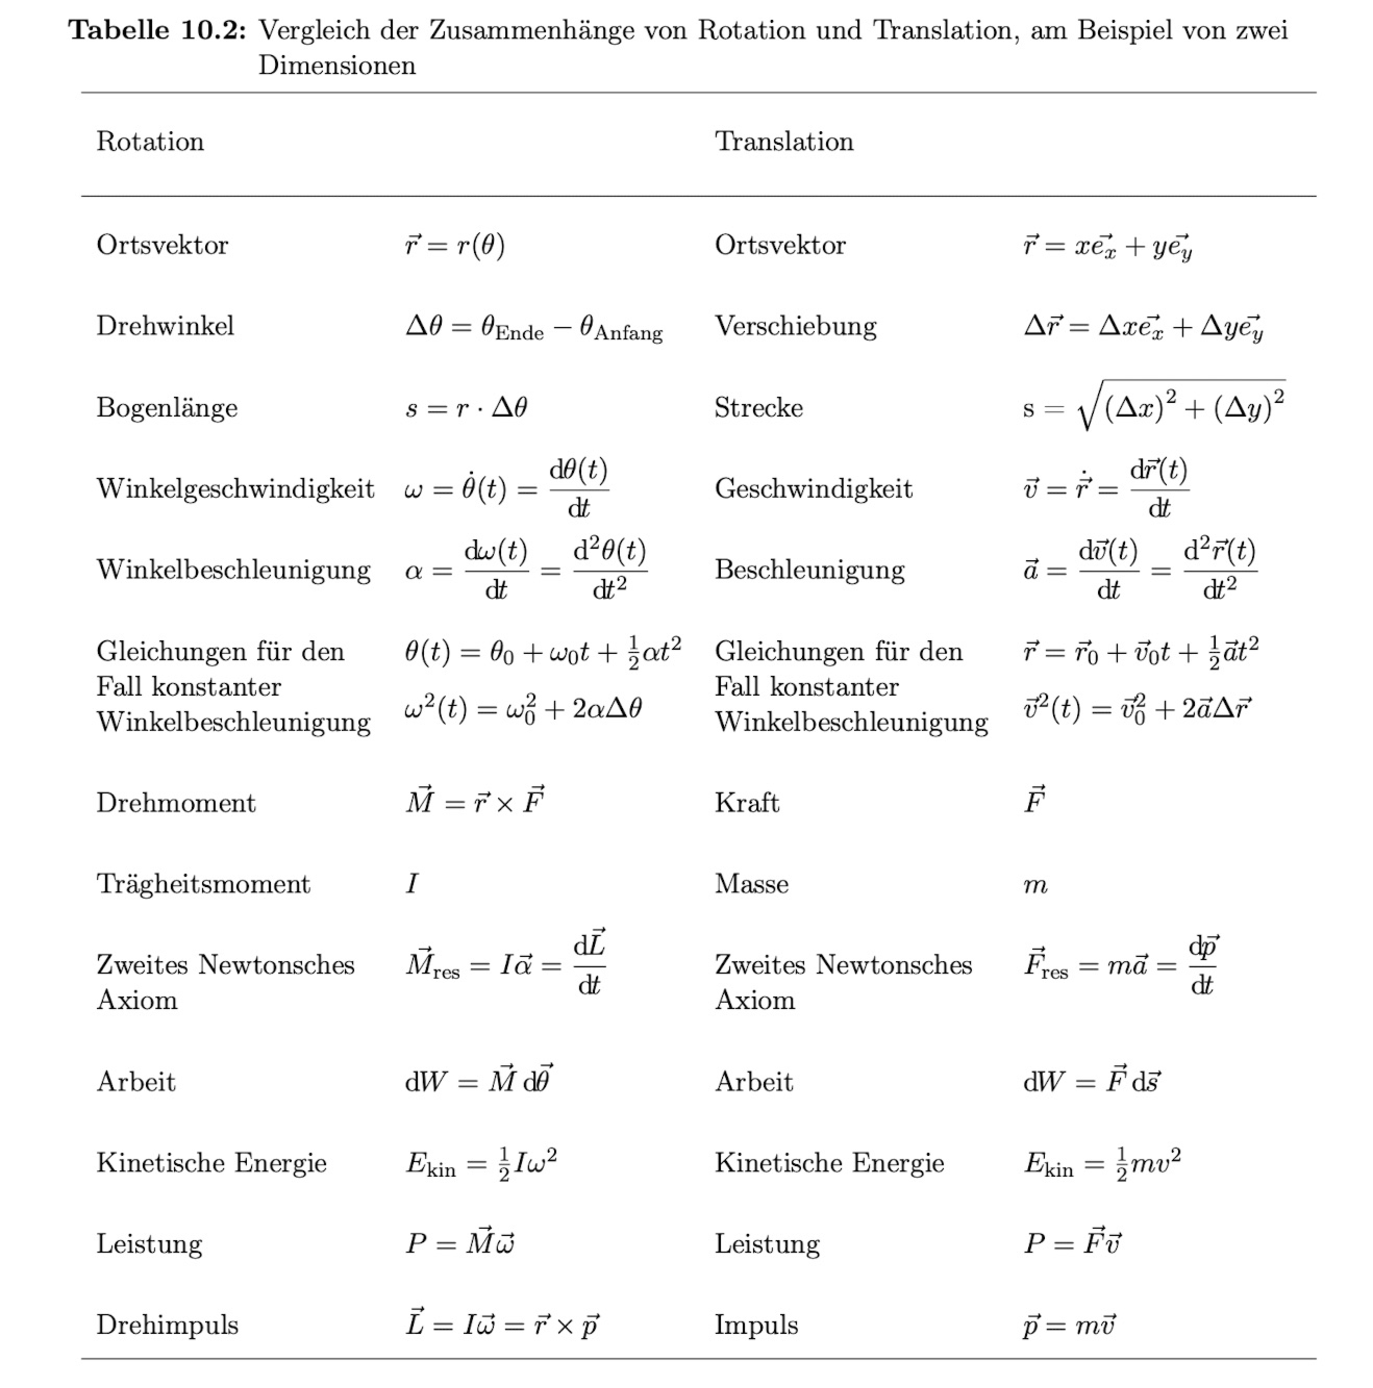
\includegraphics[width=\linewidth]{/Users/cematas/Documents/Physik/Formelsammlung 2/Images/Vergleich.pdf}
	\label{fig:beispiel}
\end{figure}

\section{Massenträgheitsmomente}

\begin{displayformula}
	Massenträgheitsmoment
	\[
	I = \sum \frac{1}{2} m_i r_i^2 
	\]
	\[
	I_{\text{ges}} = \sum_i I_i
	\]
\end{displayformula}
\formulalegend{
	\( I \): Trägheitsmoment eines Körpers [kg·m²], \( m_i \): Masse [kg], \( r_i \): Abstand zur Drehachse [m]
}

\begin{displayformula}
	Kontinuierliche Masseverteilungen
	\[
	I = \int r^2 \, dm
	\]
\end{displayformula}
\formulalegend{
	\( I \): Trägheitsmoment [kg·m²], \( r \): Abstand zur Drehachse [m], \( dm \): infinitesimale Masse [kg]
}
\begin{displayformula}
	Massiver, homogener Zylinder (Masse \( m \); Radius \( r_a \))
	\[
	I = \frac{1}{2} m \cdot r_a^2
	\]
\end{displayformula}
\formulalegend{
	\( I \): Trägheitsmoment [kg·m²], \( m \): Masse [kg], \( r_a \): Außenradius [m]
}

\begin{displayformula}
	Hohlzylinder (Masse \( m \); Innenradius \( r_i \); Außenradius \( r_a \))
	\[
	I = \frac{1}{2} m \cdot (r_a^2 + r_i^2)
	\]
\end{displayformula}
\formulalegend{
	\( I \): Trägheitsmoment [kg·m²], \( m \): Masse [kg], \( r_a \): Außenradius [m], \( r_i \): Innenradius [m]
}

\begin{displayformula}
	Dünnwandiger, hohler Zylinder (Radius \( r_a \))
	\[
	I = m \cdot r_a^2
	\]
\end{displayformula}
\formulalegend{
	\( I \): Trägheitsmoment [kg·m²], \( m \): Masse [kg], \( r_a \): Radius [m]
}

\begin{displayformula}
	Dünner Stab (Länge \( l \); durch die Mitte gedreht)
	\[
	I = \frac{1}{12} m \cdot l^2
	\]
\end{displayformula}
\formulalegend{
	\( I \): Trägheitsmoment [kg·m²], \( m \): Masse [kg], \( l \): Länge [m]
}

\begin{displayformula}
	Dünner Stab (Drehachse durch das Ende)
	\[
	I = \frac{1}{3} m \cdot l^2
	\]
\end{displayformula}
\formulalegend{
	\( I \): Trägheitsmoment [kg·m²], \( m \): Masse [kg], \( l \): Länge [m]
}

\begin{displayformula}
	Bei versetzter Drehachse
	\[
	E_{\text{kin}} = \frac{1}{2} I_s \omega^2 + \frac{1}{2} m r^2 \omega^2 = \frac{1}{2} (I_s + m r^2) \omega^2
	\]
	Steiner
	\[
	I_p = I_s + m r^2
	\]
\end{displayformula}
\formulalegend{
	\( E_{\text{kin}} \): Kinetische Energie der Rotation [J], \( I_s \): Trägheitsmoment um Schwerpunktachse [kg·m²], \( I_p \): Trägheitsmoment um Parallelachse [kg·m²], \( m \): Masse [kg], \( r \): Abstand der Achsen [m], \( \omega \): Winkelgeschwindigkeit [rad/s]
}

\section{Das zweite Newtonsche Axiom für Drehbewegungen}

\begin{displayformula}
	\[
	\vec{M} = I \cdot \vec{\alpha}
	\]
\end{displayformula}
\formulalegend{
	\( \vec{M} \): Drehmoment [Nm], \( I \): Trägheitsmoment [kg·m²], \( \vec{\alpha} \): Winkelbeschleunigung [rad/s²]
}

\begin{displayformula}
	Drehmoment über Kreuzprodukt
	\[
	\vec{M} = \vec{r} \times \vec{F}
	\]
\end{displayformula}
\formulalegend{
	\( \vec{M} \): Drehmoment [Nm], \( \vec{r} \): Hebelarm [m], \( \vec{F} \): Kraft [N]
}

\begin{displayformula}
	Tangentialbeschleunigung
	\[
	a_t = \vec{\alpha} \cdot \vec{r} \quad \Rightarrow \quad \vec{F} = m \cdot \vec{\alpha} \times \vec{r}
	\]
\end{displayformula}
\formulalegend{
	\( a_t \): Tangentialbeschleunigung [m/s²], \( \vec{\alpha} \): Winkelbeschleunigung [rad/s²], \( \vec{r} \): Radiusvektor [m], \( \vec{F} \): Kraft [N], \( m \): Masse [kg]
}

\subsection{Statisches Gleichgewicht}

\begin{displayformula}
	\[
	\vec{F} = m \cdot \vec{a} = 0
	\]
	\[
	\vec{M} = I \cdot \vec{\alpha} = 0
	\]
\end{displayformula}
\formulalegend{
	Statische Bedingungen: keine Beschleunigung, keine Winkelbeschleunigung. Kräfte- und Momentengleichgewicht.\\
	\( \vec{F} \): resultierende Kraft [N], \( \vec{a} \): Beschleunigung [m/s²], \( \vec{M} \): Drehmoment [Nm], \( \vec{\alpha} \): Winkelbeschleunigung [rad/s²]
}

\subsection{Die kinetische Energie rollender Körper}

\begin{displayformula}
	Ein rollender Körper besitzt sowohl kinetische Energie durch die Rotation, als auch kinetische Energie durch die Bewegung seines Schwerpunkts in Folge des Abrollens. \\ 
	Gesamtenergie:
	\[
	E_{\text{kin}} = \frac{1}{2} I_S \omega^2 + \frac{1}{2} m v_S^2
	\]
\end{displayformula}
\formulalegend{
	\( E_{\text{kin}} \): Gesamtenergie [J], \( I_S \): Trägheitsmoment um Schwerpunkt [kg·m²], \( \omega \): Winkelgeschwindigkeit [rad/s], \( m \): Masse [kg], \( v_S \): Schwerpunktsgeschwindigkeit [m/s]
}

\begin{displayformula}
	Vollzylinder auf schiefer Ebene (Neigung \( \beta \)):
	\[
	E_{\text{pot}} = E_{\text{kin}}
	\]
	Geschwindigkeit nach Strecke \( x \):
	\[
	v_x^2 = \frac{4}{3} g \cdot x \cdot \sin\beta
	\]
	Beschleunigung:
	\[
	a = \frac{2}{3} g \cdot \sin\beta
	\]
\end{displayformula}
\formulalegend{
	\( E_{\text{pot}} \): Potentielle Energie [J], \( v_x \): Geschwindigkeit [m/s], \( g \): Erdbeschleunigung [m/s²], \( x \): zurückgelegte Strecke [m], \( \beta \): Neigungswinkel [rad], \( a \): Beschleunigung [m/s²]
}

\section{Drehimpuls und Drehimpulserhaltung}

\begin{displayformula}
	Drehimpuls
	\[
	L = I \cdot \omega = \vec{r} \times \vec{p}
	\]
	\[
	\vec{L}_{\text{ges}} = \vec{L}_{\text{Bahn}} + \vec{L}_{\text{Spin}} = m \cdot \vec{r}_S \times \vec{v}_S + \vec{L}_{\text{Spin}}
	\]
\end{displayformula}
\formulalegend{
	\( L \): Drehimpuls [kg·m²/s], \( I \): Trägheitsmoment [kg·m²], \( \omega \): Winkelgeschwindigkeit [rad/s], \( \vec{r} \): Ort [m], \( \vec{p} \): Impuls [kg·m/s], \( \vec{v}_S \): Geschwindigkeit Schwerpunkt [m/s]
}

\begin{displayformula}
	Drehimpulserhaltung
	\[
	\vec{L}_{\text{ges}} = \sum_i I_i \cdot \omega_i = \text{konstant}, \quad \text{wenn } \vec{M}_{\text{ges}} = 0
	\]
\end{displayformula}
\formulalegend{
	\( \vec{L}_{\text{ges}} \): Gesamtdrehimpuls [kg·m²/s], \( \vec{M}_{\text{ges}} \): Summe der äußeren Drehmomente [Nm]
}

\section{Schwingungen}

\subsection{Ungedämpfte, freie und harmonische Schwingungen}

\begin{displayformula}
	Auslenkung, Geschwindigkeit, Beschleunigung
	\[
	y(t) = A \cdot \cos(\omega_0 t + \delta)
	\]
	\[
	v(t) = -\omega_0 A \cdot \sin(\omega_0 t + \delta)
	\]
	\[
	a(t) = -\omega_0^2 A \cdot \cos(\omega_0 t + \delta)
	\]
\end{displayformula}
\formulalegend{
	\( y(t) \): Auslenkung [m], \( v(t) \): Geschwindigkeit [m/s], \( a(t) \): Beschleunigung [m/s²], \( A \): Amplitude [m], \( \omega_0 \): Kreisfrequenz [rad/s], \( \delta \): Phasenverschiebung [rad], \( t \): Zeit [s]
}

\begin{displayformula}
	Kreisfrequenz
	\[
	\omega_0 = 2\pi f_0 = \frac{2\pi}{T_0} = \sqrt{\frac{k_F}{m}}
	\]
\end{displayformula}
\formulalegend{
	\( \omega_0 \): Kreisfrequenz [rad/s], \( f_0 \): Frequenz [Hz], \( T_0 \): Periodendauer [s], \( k_F \): Federkonstante [N/m], \( m \): Masse [kg]
}

\begin{displayformula}
	Energie des harmonischen Oszillators
	\[
	E_{\text{mech}} = \frac{1}{2} k_F \cdot A^2
	\]
\end{displayformula}
\formulalegend{
	\( E_{\text{mech}} \): Mechanische Energie [J], \( k_F \): Federkonstante [N/m], \( A \): Amplitude [m]
}

\begin{displayformula}
	Vertikaler Federschwinger
	\[
	\omega_0 = \sqrt{\frac{k_F}{m}}
	\]
\end{displayformula}
\formulalegend{
	\( \omega_0 \): Kreisfrequenz [rad/s], \( k_F \): Federkonstante [N/m], \( m \): Masse [kg]
}

\begin{displayformula}
	Mathematisches Pendel
	\[
	\ddot{\theta}(t) + \frac{g}{l} \sin\theta(t) = 0
	\]
	Linearisiert:
	\[
	\ddot{\theta}(t) + \frac{g}{l} \theta(t) = 0
	\]
	\[
	\omega_0 = \sqrt{\frac{g}{l}}
	\]
\end{displayformula}
\formulalegend{
	\( \theta(t) \): Winkel [rad], \( g \): Erdbeschleunigung [m/s²], \( l \): Pendellänge [m], \( \omega_0 \): Kreisfrequenz [rad/s]
}

\begin{displayformula}
	Drehpendel / Torsionspendel
	\[
	\ddot{\theta}(t) + \frac{\kappa}{I} \theta(t) = 0
	\quad \Rightarrow \quad \omega_0 = \sqrt{\frac{\kappa}{I}}
	\]
\end{displayformula}
\formulalegend{
	\( \theta(t) \): Auslenkwinkel [rad], \( \kappa \): Drehfederkonstante [Nm], \( I \): Trägheitsmoment [kg·m²]
}

\begin{displayformula}
	Physikalisches Pendel
	\[
	\ddot{\theta}(t) + \frac{s m g}{I_p} \sin\theta(t) = 0
	\quad \Rightarrow \quad \omega_0 = \sqrt{\frac{s m g}{I_p}}
	\]
\end{displayformula}
\formulalegend{
	\( \theta(t) \): Winkel [rad], \( s \): Abstand zur Drehachse [m], \( m \): Masse [kg], \( g \): Erdbeschleunigung [m/s²], \( I_p \): Trägheitsmoment bezogen auf Drehachse [kg·m²]
}

\begin{displayformula}
	Elastischer Schwingkreis
	\[
	\ddot{Q}(t) + \frac{1}{LC} Q(t) = 0
	\quad \Rightarrow \quad \omega_0 = \sqrt{\frac{1}{LC}}
	\]
\end{displayformula}
\formulalegend{
	\( Q(t) \): Ladung [C], \( L \): Induktivität [H], \( C \): Kapazität [F], \( \omega_0 \): Kreisfrequenz [rad/s]
}


\subsection{Gedämpfte Schwingungen}

\begin{displayformula}
	DGL für Feder-Masse-Dämpfungssystem:
	\[
	\ddot{y}(t) + 2\delta \dot{y}(t) + \omega_0^2 y(t) = 0
	\quad \text{mit } 2\delta = \frac{b}{m}
	\]
\end{displayformula}
\formulalegend{
	\( y(t) \): Auslenkung [m], \( \delta \): Abklingkonstante [1/s], \( b \): Dämpfungskonstante [kg/s], \( m \): Masse [kg], \( \omega_0 \): ungedämpfte Kreisfrequenz [rad/s]
}

\begin{displayformula}
	Dämpfungsgrad
	\[
	D = \frac{\delta}{\omega_0}
	\]
\end{displayformula}
\formulalegend{
	\( D \): Dämpfungsgrad, \( \delta \): Abklingkonstante [1/s], \( \omega_0 \): Kreisfrequenz [rad/s]
}

\begin{displayformula}
	Lösung der charakteristischen Gleichung
	\[
	\lambda_{1,2} = -\delta \pm \sqrt{\delta^2 - \omega_0^2}
	\]
\end{displayformula}
\formulalegend{
	\( \lambda \): Eigenwerte, \( \delta \): Abklingkonstante [1/s], \( \omega_0 \): Kreisfrequenz [rad/s]
}

\begin{figure}[h!]
	\centering
	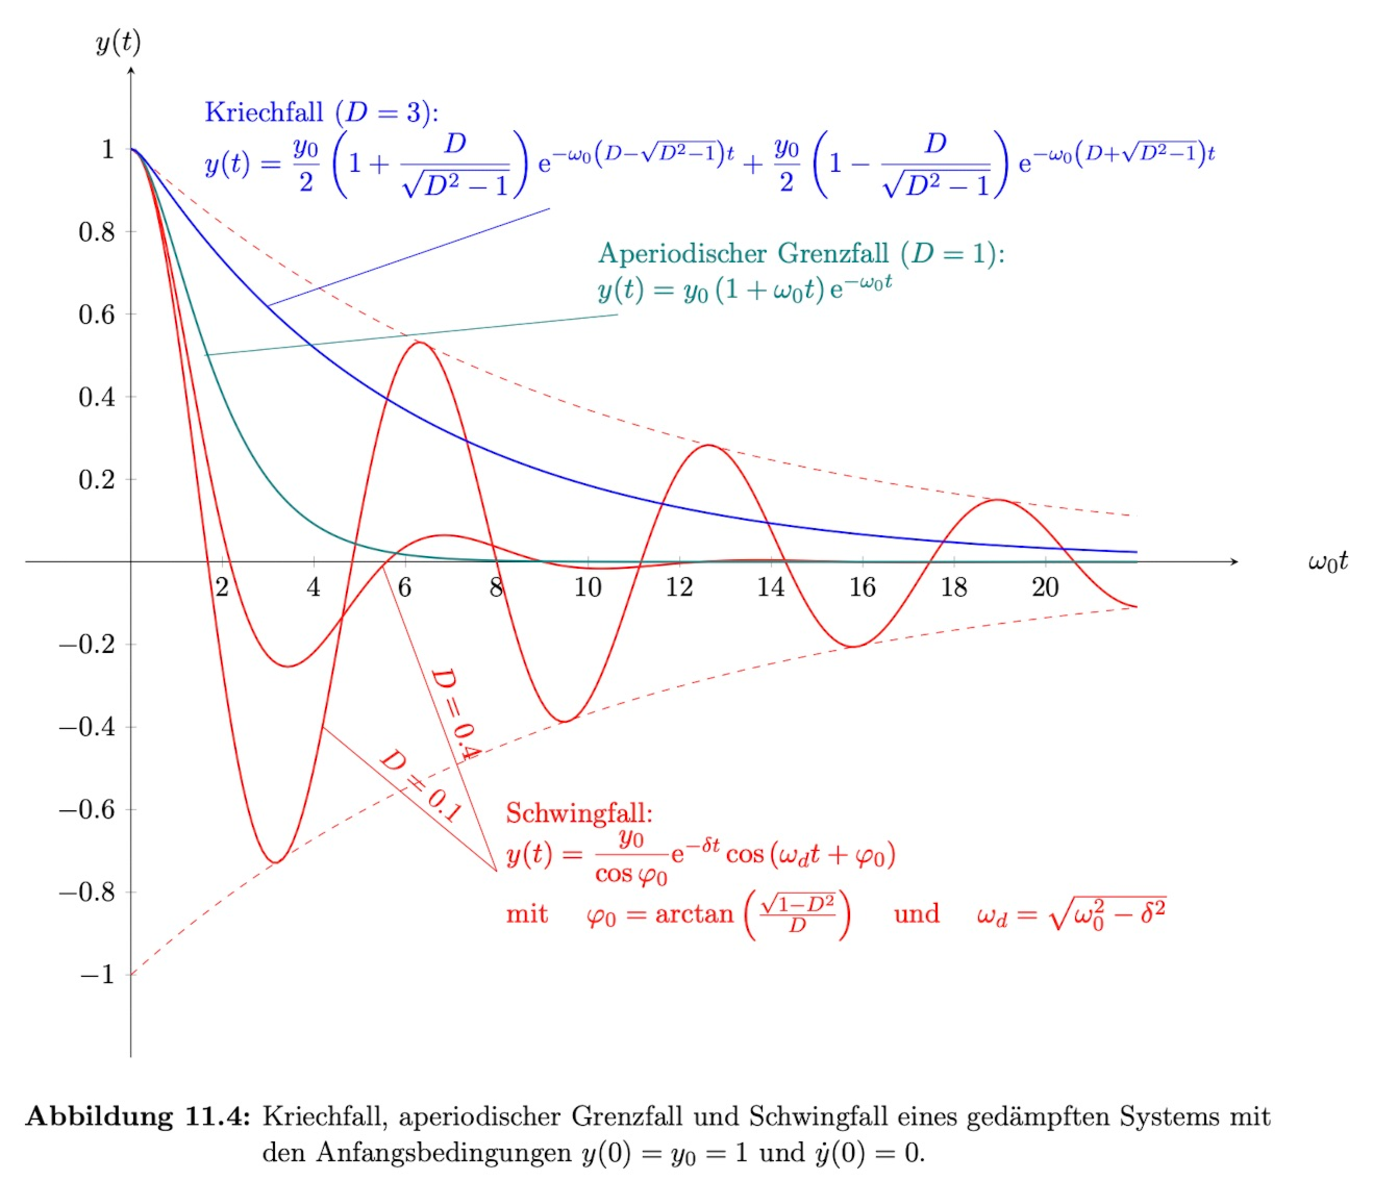
\includegraphics[width=\linewidth]{/Users/cematas/Documents/Physik/Formelsammlung 2/Images/DGL.pdf}
\end{figure}

\subsection{Energie des gedämpften Oszillators}

\begin{displayformula}
	Schwach gedämpft (Näherung \( \omega_d \approx \omega_0 \)):
	\[
	E_{\text{mech}} = \frac{1}{2} m \cdot \omega_0^2 \cdot A^2
	\]
\end{displayformula}
\formulalegend{
	\( E_{\text{mech}} \): Energie [J], \( m \): Masse [kg], \( \omega_0 \): Kreisfrequenz [rad/s], \( A \): Amplitude [m]
}

\begin{displayformula}
	Stärker gedämpft:
	\[
	E_{\text{mech}} = \frac{1}{2} m \cdot \omega_d^2 \cdot A^2
	\]
\end{displayformula}
\formulalegend{
	\( \omega_d \): gedämpfte Eigenfrequenz [rad/s]
}

\subsection{Güte}

\begin{displayformula}
	Gütefaktor
	\[
	Q = \frac{1}{2D} = \omega_0 \cdot \frac{m}{b}
	\]
\end{displayformula}
\formulalegend{
	\( Q \): Gütefaktor, \( D \): Dämpfungsgrad, \( \omega_0 \): Kreisfrequenz [rad/s], \( m \): Masse [kg], \( b \): Dämpfungskonstante [kg/s]
}

\section{Wellen}

\begin{displayformula}
	Eindimensionale Wellengleichung
	\[
	\frac{\partial^2 y(z,t)}{\partial t^2} = \frac{F_s}{A \rho} \cdot \frac{\partial^2 y(z,t)}{\partial z^2}
	\]
\end{displayformula}
\formulalegend{
	\( y(z,t) \): Auslenkung [m], \( F_s \): Zugkraft [N], \( A \): Querschnittsfläche [m²], \( \rho \): Dichte [kg/m³]
}

\begin{displayformula}
	Lösung der harmonischen Wellenfunktion
	\[
	y(z, t) = A \cdot \cos(\omega t - kz + \delta)
	\]
	\[
	k = \frac{2\pi}{\lambda}, \quad c = \frac{\lambda}{T} = \frac{\omega}{k} = \nu \cdot \lambda
	\]
\end{displayformula}
\formulalegend{
	\( y(z,t) \): Auslenkung [m], \( A \): Amplitude [m], \( \omega \): Kreisfrequenz [rad/s], \( k \): Wellenzahl [rad/m], \( \delta \): Phase [rad], \( \lambda \): Wellenlänge [m], \( T \): Periodendauer [s], \( \nu \): Frequenz [Hz], \( c \): Ausbreitungsgeschwindigkeit [m/s]
}


\begin{displayformula}
	Phasengeschwindigkeit verschiedener Wellen \\ 
	Seilwellen
	\[
	c = \sqrt{\frac{F_s}{\mu}}
	\]
		\[
	\mu = \frac{m}{l}
	\]
	Elektromagnetische Wellen im Vakuum
	\[
	c = \frac{1}{\sqrt{\epsilon_0 \mu_0}}
	\]
	Elektromagnetische Wellen in Materie
	\[
	c = \frac{1}{\sqrt{\epsilon_r \epsilon_0 \mu_r \mu_0}}
	\]
\end{displayformula}
\formulalegend{
	\( c \): Phasengeschwindigkeit [m/s], 
	\( F_s \): Spannkraft im Seil [N], 
	\( \mu \): lineare Massendichte [kg/m], 
	\( \epsilon_0 \): elektrische Feldkonstante (Permittivität des Vakuums) [F/m], 
	\( \mu_0 \): magnetische Feldkonstante (Permeabilität des Vakuums) [H/m], 
	\( \epsilon_r \): relative Permittivität, 
	\( \mu_r \): relative Permeabilität,
	\(m\): masse [kg],
	\(l\): länge [l]
	\}
}

\subsection{Wellen in drei Dimensionen}
\begin{displayformula}
	Intensität:
	\[
	I(z) = \frac{\text{zeitlich gemittelte Lieistung}}{\text{senkrecht zur Ausbreitung stehende Fläche}} = \frac{P_t}{A} = \text{const.}
	\]
	Kreiswellen
	\[
	I(r) = \frac{I_0r_0}{r}
	\]
	Kugelwellen
	\[
	I(r) = \frac{I_0r_0^2}{r^2} = \frac{P_t}{4\pi r^2}
	\]
\end{displayformula}
\formulalegend{
	\( I(z), I(r) \): Intensität [W/m\(^2\)], 
	\( P_t \): zeitlich gemittelte Leistung [W], 
	\( A \): Fläche senkrecht zur Ausbreitungsrichtung [m\(^2\)], 
	\( I_0 \): Referenzintensität in Abstand \( r_0 \) [W/m\(^2\)], 
	\( r, r_0 \): Abstand zur Quelle bzw. Referenzabstand [m]
}

\begin{displayformula}
	Messung der Schallintensität
	\[
	I_p = 10\log \frac{I}{I_0} \text{dB}
	\]
\end{displayformula}
\formulalegend{
	$I_p$: Schalldruckpegel [dB], 
	$I$: gemessene Schallintensität [W/m$^2$], 
	$I_0$: Bezugsintensität, meist $10^{-12}$ W/m$^2$
}



\subsection{Der Doppler-Effekt}

\begin{displayformula}
	Fall 1: Empfänger bewegt sich relativ zu einer still stehenden Quelle
	\[
	\nu_E = \nu_0 (1 \textcolor{blue}{+} / \textcolor{red}{-} \frac{V_E}{c})
	\]
	\textcolor{blue}{Hinbewegung} \\
	\textcolor{red}{Wegbewegung}
\end{displayformula}

\begin{displayformula}
	Fall 2: Quelle bewegt sich relativ zu einem still stehenden Empfänger
	\[
	\nu_E = \nu_0 \frac{1}{1 \textcolor{red}{-} / \textcolor{blue}{+} \frac{V_Q}{c}}
	\]
	\textcolor{red}{Hinbewegung} \\
	\textcolor{blue}{Wegbewegung}
\end{displayformula}

\begin{displayformula}
	Fall 3: Quelle und Empfänger bewegen sich relativ zueinander
	\[
	\nu_E = \frac{1 \textcolor{red}{+} / \textcolor{blue}{-} \frac{V_E}{c}}{1 \textcolor{red}{-} / \textcolor{blue}{+} \frac{V_Q}{c}}
	\]
	\textcolor{red}{Hinbewegung} \\
	\textcolor{blue}{Wegbewegung}
\end{displayformula}

\formulalegend{
	$\nu_E$: Frequenz beim Empfänger [Hz], 
	$\nu_0$: Frequenz der Quelle [Hz], 
	$V_E$: Geschwindigkeit des Empfängers relativ zum Medium [m/s], 
	$V_Q$: Geschwindigkeit der Quelle relativ zum Medium [m/s], 
	$c$: Ausbreitungsgeschwindigkeit der Welle im Medium [m/s], 
}

\begin{displayformula}
	Fall 4: Entstehung von Stoßwellen
	\[
	\sin \theta = \frac{c}{V_Q} = \frac{1}{\text{Ma}}
	\]
\end{displayformula}

\section{Überlagerung von Wellen}

\subsection{Überlagerung von zwei Wellen mit gleicher Wellenzahl und Frequenz}
\begin{displayformula}
\[
y_1 = A \cos (kz - \omega t)
\]
\[
y_2 = A \cos (kz - \omega t + \delta)
\]
\[
y = y_1 + y_2
\]
\[
y = 2 A \cos (\frac{1}{2} \delta) \cos (kz - \omega t + \frac{1}{2} \delta)
\]
\end{displayformula}
Der erste Teil der Formel ($2A \cos (\frac{1}{2} \delta$) stellt die resultierende Amplitude $A_{res}$ dar. \\
Der Zweite Teil der Formel ($\cos (kz - \omega t + \frac{1}{2} \delta)$) beschreibt die, sich in Z-Richtung ausbreitende Welle

\begin{displayformula}
	Gangunterschied
	\[
	\Delta z = \frac{\delta}{2 \pi} \lambda
	\]
	
	\[
	\Delta z = z_2 - z_1
	\]
\end{displayformula}
Der Gangunterschied stellt anschaulich den räumlichen Versatz der beiden Wellen in Bezug auf die Wellenlänge $\lambda$ dar
\formulalegend{
	$y_1$, $y_2$: Einzelne Wellenfunktionen, 
	$y$: resultierende Welle, 
	$A$: Amplitude der Einzelsignale, 
	$A_{\text{res}} = 2A \cos(\frac{1}{2}\delta)$: resultierende Amplitude, 
	$k$: Wellenzahl, $k = \frac{2\pi}{\lambda}$ [$\text{rad}/\text{m}$], 
	$\omega$: Kreisfrequenz, $\omega = 2\pi f$ [$\text{rad}/\text{s}$], 
	$f$: Frequenz [Hz], 
	$\delta$: Phasendifferenz [rad], 
	$\lambda$: Wellenlänge [m], 
	$\Delta z$: Gangunterschied [m], 
	$z_1$, $z_2$: Orte der beiden Wellenfronten
}



\subsection{Interferenzbedingungen}

\textbf{Konstruktive Interferenz}

\begin{itemize}
	\item \textbf{Phasenkonstante:} $\delta = 0,\ \pm 2\pi,\ \pm 4\pi,\ \dots$
	\item \textbf{Gangunterschied:} $\Delta z = 0,\ \pm \lambda,\ \pm 2\lambda,\ \dots$
	\item \textbf{Ergebnis:} Verstärkung der Wellen (Maxima überlagern sich)
\end{itemize}

\vspace{1ex}

\textbf{Destruktive Interferenz}

\begin{itemize}
	\item \textbf{Phasenkonstante:} $\delta = \pm \pi,\ \pm 3\pi,\ \pm 5\pi,\ \dots$
	\item \textbf{Gangunterschied:} $\Delta z = \pm \frac{\lambda}{2},\ \pm \frac{3\lambda}{2},\ \pm \frac{5\lambda}{2},\ \dots$
	\item \textbf{Ergebnis:} Auslöschung der Wellen (Maxima und Minima überlagern sich)
\end{itemize}

\subsection{Überlagerung von zwei Wellen mit geringfügig unterschiedlicher Frequenz und Wellenlänge}

\begin{displayformula}
	\[
	y_1 = A \cos (k_1z - \omega_1 t)
	\]
	\[
	y_2 = A \cos (k_2z - \omega_2 t)
	\]
	\[
	y = y_1 + y_2
	\]
	\[
	y = 2 A \cos (\frac{1}{2} \Delta kz - \frac{1}{2} \Delta \omega t) \cos (\frac{(k_1 + k_2)}{2} z - \frac{(\omega_1 + \omega_2)}{2}t)
	\]
\end{displayformula}
Der erste Teil der Formel ($2 A \cos (\frac{1}{2} \Delta kz - \frac{1}{2} \Delta \omega t)$) stellt die resultierende Amplitude $A_{res}$ dar. \\
Der Zweite Teil der Formel ($\cos (\frac{(k_1 + k_2)}{2} z - \frac{(\omega_1 + \omega_2)}{2}t)$) beschreibt die, sich in Z-Richtung ausbreitende Welle

Wenn die Differenz 1Hz beträgt, hat man jede Sekunde ein Auf- und Abklingen ($\frac{1}{1 Hz} = 1s$). Bei 3 Hz hat man schon 3 Auf- und Abklingen pro Sekunde
\formulalegend{
	$y_1$, $y_2$: Einzelne Wellenfunktionen, 
	$y$: resultierende Welle, 
	$A$: Amplitude der Einzelsignale, 
	$A_{\text{res}}$:  resultierende Amplitude, 
	$k$: Wellenzahl, $k = \frac{2\pi}{\lambda}$ [$\text{rad}/\text{m}$], 
	$\omega$: Kreisfrequenz, $\omega = 2\pi f$ [$\text{rad}/\text{s}$], 
	$f$: Frequenz [Hz], 
	$\delta$: Phasendifferenz [rad], 
	$\lambda$: Wellenlänge [m], 
	$\Delta z$: Gangunterschied [m], 
	$z_1$, $z_2$: Orte der beiden Wellenfronten
}

\begin{displayformula}
		Ausbreitungsgeschwindigkeit des Wellenpakets (Gruppengeschwindigkeit):
	\[
	v_{gr} = \frac{\Delta \omega}{\Delta k} = \frac{c}{n_{gr}}
	\]
\end{displayformula}
\formulalegend{
	\( v_{gr} \): Gruppengeschwindigkeit [m/s],
	\( \Delta \omega \): Änderung der Kreisfrequenz [rad/s],
	\( \Delta k \): Änderung der Wellenzahl [1/m],
	\( c \): Lichtgeschwindigkeit im Vakuum [m/s],
	\( n_{gr} \): Gruppengeschwindigkeitsbrechungsindex [–]
}


\begin{displayformula}
		Phasengeschwindigkeit
	\[
	v_{ph} = \frac{\bar{ \omega}}{\bar{k}} = \frac{c}{\bar{n}}
	\]
\end{displayformula}
\formulalegend{
	\( v_{ph} \): Phasengeschwindigkeit [m/s], 
	\( \bar{\omega} \): mittlere Kreisfrequenz [rad/s], 
	\( \bar{k} \): mittlere Wellenzahl [1/m], 
	\( c \): Lichtgeschwindigkeit im Vakuum [m/s], 
	\( \bar{n} \): Brechzahl
}


\section{Reflexion und Transmission an Grenzschichten}

\begin{displayformula}
Bei Seilkraft gilt: 
	\[
	c = \sqrt{\frac{F_s}{\mu}}
	\]
	\[
	\mu = \frac{m}{l}
	\]
\end{displayformula}
\formulalegend{
	\( c \): Wellengeschwindigkeit auf dem Seil [m/s], 
	\( F_s \): Seilkraft (Zugspannung) [N], 
	\( \mu \): lineare Massendichte [kg/m], 
	\( m \): Masse des Seils [kg], 
	\( l \): Länge des Seils [m]
}


\begin{displayformula}
	Die Amplituden der reflektierten und transmittierten Welle ergeben sich mit Hilfe des \\ Reflektionskoeffizienten R
	\[
	y_R = R \cdot y_0 = \frac{c_2 - c_1}{c_2 + c_1} \cdot y_0 = \frac{n_1 - n_2}{n_1 + n_2} \cdot y_0
	\]
	Und dem Transmissionskoeffizienten T
	\[
	y_T = T \cdot y_0 = \frac{2c_2}{c_2 + c_1} \cdot y_0 = \frac{2n_1}{n_1 + n_2} \cdot y_0
	\]
\end{displayformula}
\formulalegend{
	\( y_R \): Amplitude der reflektierten Welle [m], 
	\( y_T \): Amplitude der transmittierten Welle [m], 
	\( y_0 \): Amplitude der einfallenden Welle [m], 
	\( R \): Reflektionskoeffizient [–], 
	\( T \): Transmissionskoeffizient [–], 
	\( c_1 \), \( c_2 \): Wellengeschwindigkeiten in Medium 1 bzw. 2 [m/s], 
	\( n_1 \), \( n_2 \): Brechungsindizes der beiden Medien [–]
}

Durch R wird die Amplitude der reflektierten Welle berechnet. Ist diese negativ, startet die Amplitude am Reflexionspunkt beim negativen Wert des berechneten R. \\
Durch T wird die Amplitude der transmittierten Welle berechnet. Selbe Logik wie bei R. \\
Zwei Wellen können sich auch gegenseitig auslöschen, wenn die Amplituden gleich groß und entgegengesetzt sind.

\begin{displayformula}
	Bei Energieübertragung, der Wellenintensität (elektromagnetische Wellen, Licht): \\
	Reflexionsgrad $\rho$ = $R^2$
	\[
	I_R = \rho \cdot I_0 = (\frac{c_2 - c_1}{c_2 + c_1})^2 \cdot I_0 = (\frac{n_1 - n_2}{n_1 + n_2})^2 \cdot I_0
	\]
	Und dem Transmissionsgrad $\tau$ =  $1 - \rho$
	\[
	I_T = \tau \cdot I_0 = \frac{4n_1n_2}{(n_1 + n_2)^2} \cdot I_0
	\]
\end{displayformula}
\formulalegend{
	\( I_R \): Intensität der reflektierten Welle [W/m²], 
	\( I_T \): Intensität der transmittierten Welle [W/m²], 
	\( I_0 \): Intensität der einfallenden Welle [W/m²], 
	\( \rho \): Reflexionsgrad [–], 
	\( \tau \): Transmissionsgrad [–], 
	\( R \): Reflektionskoeffizient [–], 
	\( c_1 \), \( c_2 \): Wellengeschwindigkeiten in Medium 1 bzw. 2 [m/s], 
	\( n_1 \), \( n_2 \): Brechungsindizes der beiden Medien [–]
}


\section{Stehende Wellen}

\subsection{Stehende Wellen bei beidseitig gleichartigen Enden}

\begin{displayformula}
	Die Bedingung für eine stehende Welle bei beidseitig gleichartiger Begrenzung lautet:
	\[
	L = n\frac{\lambda_n}{2} \text{mit n = 1, 2, 3, ...}
	\]
	Dadurch ergeben sich die Resonanzfrequenzen
	\[
	\nu_n = \frac{n}{2} \cdot \frac{c}{L} = n \cdot \nu_1 \text{mit n = 1, 2, 3, ...}
	\]
	Der Abstand benachbarter Resonanzfrequenzen entspricht der Grundresonanzfrequenz
	\[
	\Delta_\nu = \nu_1
	\]
\end{displayformula}


\subsection{Stehende Wellen bei unterschiedlicher (z.B.) einseitiger Begrenzung}

\begin{displayformula}
	Die Bedingung für eine stehende Welle bei unterschiedlicher Begrenzung lautet:
	\[
	L = n\frac{\lambda_n}{4} \text{mit n = 1, 3, 5, ...}
	\]
	Dadurch ergeben sich die Resonanzfrequenzen
	\[
	\nu_n = \frac{n}{4} \cdot \frac{c}{L} = n \cdot \nu_1 \text{mit n = 1, 3, 5, ...}
	\]
	Der Abstand benachbarter Resonanzfrequenzen entspricht dem doppelten der Grundresonanzfrequenz
	\[
	\Delta_\nu = 2\nu_1
	\]
\end{displayformula}
\formulalegend{
	\( L \): Länge des schwingenden Mediums [m], 
	\( \lambda_n \): Wellenlänge der \(n\)-ten stehenden Welle [m], 
	\( n \): Ordnung, 
	\( \nu_n \): Frequenz der \(n\)-ten Resonanz [Hz], 
	\( \nu_1 \): Grundresonanzfrequenz [Hz], 
	\( \Delta_\nu \): Frequenzabstand benachbarter Resonanzen [Hz], 
	\( c \): Ausbreitungsgeschwindigkeit der Welle [m/s]
}


\section{Optik}

\subsection{Wellengleichung}

\begin{displayformula}
	Ausbreitungsgeschwindigkeit von elektromagnetischen Wellen:
	\[
	C = \frac{1}{\sqrt{\mu_0 \epsilon_0} \cdot \sqrt{\mu_r \epsilon_r}} = \frac{C_0}{n}
	\]
	\[
	C_0 \approx 3 \cdot 10^8 \frac{m}{s}
	\]
	\[
	n = \sqrt{\mu_r \epsilon_r}
	\]
\end{displayformula}
\formulalegend{
	\( C \): Ausbreitungsgeschwindigkeit der elektromagnetischen Welle im Medium [m/s], 
	\( C_0 \): Lichtgeschwindigkeit im Vakuum [m/s], 
	\( \mu_0 \): magnetische Feldkonstante (Permeabilität des Vakuums) [H/m], 
	\( \epsilon_0 \): elektrische Feldkonstante (Permittivität des Vakuums) [F/m], 
	\( \mu_r \): relative Permeabilität des Mediums [–], 
	\( \epsilon_r \): relative Permittivität des Mediums [–], 
	\( n \): Brechzahl
}


\subsection{Eigenschaften des Lichts}

\begin{displayformula}
	Trifft Licht auf ein Medium, so ändert sich nicht die Frequenz des Lichts, sondern die Wellenlänge und beträgt:
	\[
	\lambda_{Med} = \frac{C}{\mu} = \frac{\frac{C_0}{n}}{\mu} = \frac{\lambda}{n}
	\]
	Fall a) Bei Abmessungen <= $\lambda$: \\
	\begin{itemize}
		\item Ausbreitung von Licht muss mit Maxwellschen Wellengleichungen betrachtet werden 
		\item Licht erfährt beim Auftrefen auf Grenzschichten und Gegenständen Effekte wie Interferenz und Beugung \\
	\end{itemize}
	
	Fall b) Geometrische Optik bei Abmessungen > $\lambda$: \\
	\begin{itemize}
		\item Verwendung des Strahlenmodells: Licht breitet sich in der geometrischen Optik im homogenen Medium geradlinig aus 
		\item Huygensches Prinzip: Jeder Punkt einer Wellenfront ist Ausgangspunkt einer neuen Elementarwelle
		\item Fermatsches Prinzip: Die Ausbreitung des Lichts erfolgt zwischen zwei Punkten im Medium auf dem Weg, füür den die benötigte Zeit ein Minimum ist.
	\end{itemize}

\end{displayformula}
\formulalegend{
	\( \lambda_{Med} \): Wellenlänge des Lichts im Medium [m], 
	\( C \): Lichtgeschwindigkeit im Medium [m/s], 
	\( C_0 \): Lichtgeschwindigkeit im Vakuum [m/s], 
	\( \mu \): Frequenz des Lichts [Hz], 
	\( n \): Brechzahl, 
	\( \lambda \): Wellenlänge des Lichts im Vakuum [m]
}


\subsection{Brechung und Reflexion}

\begin{displayformula}
	\begin{itemize}
		\item Die Ausbreitungsgeschwindigkeit elektromagnetischer Wellen ändert sich, wenn sie in ein Medium mit anderer Brechzahl übergehen
		\item Die Änderung der Ausbreitungsgeschwindigkeit spielt eine wesentliche Rolle, wenn Licht nicht senkrecht auf eine Grenzfläche trifft
	\end{itemize}
\end{displayformula}


\end{document}
